\section{Goniometria}
Todo plano en el espacio tiene una posición cero (O) o posición de inicio, y este punto es movible de acuerdo al marco de referencia o punto de vista del observador y de la medición que se quiera realizar, por ejemplo si se quisiera saber hasta que ángulo se puede girar el brazo de forma vertical, en un plano (X,y),  so coloca el punto 0 Exactamente en el hombro, siendo este el eje de rotación del brazo y partir de ahí se tienen ejes de referencia para determinar hasta que punto el movimiento es de flexión o extensión , en la figura 3, se puede observar el punto cero y el eje de de movimiento para el brazo.

\begin{figure}[H]
    \centering
    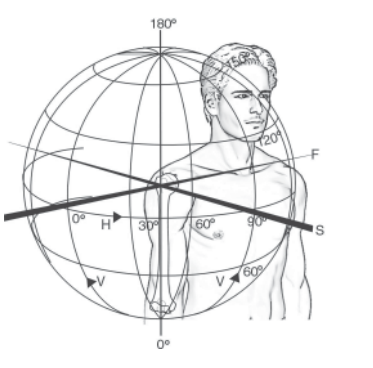
\includegraphics[width=0.5\textwidth]{Anexos/LATEX/chapters/images/ejemplo1.PNG}
    \caption{Arco de movimiento del brazo en un plano}
    \small{\textbf{Fuente:}  }
    \label{GONIOMETRIA}
\end{figure}

Si el movimiento se captura en la tiempo en un momento fijo, se puede representar como un vector $\vec{F}$ en el plano cartesiano el cual tiene una magnitud, y una inclinación ya sea vertical horizontal o inclinada, lo cual determina el ángulo al cual se está sometiendo la articulación, con estos factores magnitud y dirección se tiene un eje matemático con respecto a triángulos rectángulos donde se pueden encontrar componentes para descomponer estos vectores y así determinar los arcos de movimientos permitidos por el antebrazo, mano y muñeca.

%%% Sirve pero más adelante

%Partiendo de la necesidad de mejorar la comunicación maquina-hombre, en los últimos años se han desarrollado diferentes sensores de tipo óptico (RGB-D), que permiten una interacción natural entre el cuerpo humano y los computadores.\parencite{Grudin2017FromInteraction}\parencite{Henry200720Exploration} 

%Paralelamente, el número de aplicaciones que se desarrollan con la finalidad de afianzar esta interacción aumenta, beneficiándose especialmente de la precisión y robustez de los sensores \parencite{Khoshelham2012AccuracyApplications}. A continuación, se presentan las herramientas tecnológicas más precisas con las cuales se llevará a cabo el proyecto.

%%% Copy pastazo

%Cuando un objeto es iluminado, se produce una reflexión de luz que llega al dispositivo e incide sobre las lentes de las dos cámaras. Estas lentes, de tipo biconvexas, concentran los rayos en el sensor de cada cámara; y los datos recogidos por los sensores se almacenan en una matriz (imagen digitalizada) en la memoria del controlador USB, en donde se realizan los ajustes de resolución adecuados mediante el microcontrolador del dispositivo, produciéndose lo que se conoce como una distorsión compleja en un plano, de tipo mapa mallado de puntos que calibrados se superponen a la imagen capturada por el sensor.

%\begin{figure}[H]
    %\centering
    %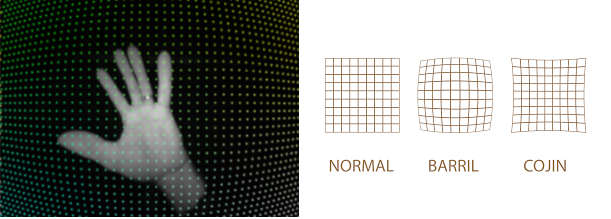
\includegraphics[width=0.8\textwidth]{Anexos/LATEX/chapters/images/complex.png}
    %\caption{Vista interna  Leap Motion y mapa mallado en plano complejo en forma de %cojín}
    %\small{\textbf{Fuente:} https://goo.gl/yuCTnk}
    %\label{LEAP2}
%\end{figure}
%El controlador Leap Motion es un sensor de nivel de consumidor de bajo costo a comparación de otros en el mercado, su precio se encuentra oscilando los \$83.89 (USD) este controlador fue desarrollado por Leap Motion (Leap Motion, http://www.leapmotion.com). Está diseñado principalmente para la detección de la posición de los dedos en aplicaciones de software interactivas. Debido a la patente actual, solo se dispone de información suficiente sobre los marcos geométricos o matemáticos del software. Sin embargo, las primeras impresiones de las capacidades de detección de posición son bastante buenas, Por lo tanto, a continuación. La Figura 1 muestra una vista esquemática de la configuración del hardware del controlador. Además de los tres emisores de infrarrojos, el dispositivo incorpora dos cámaras CCD  (Charge Coupled Device o, en español, Dispositivo de Carga Acoplada) ver Figura 1 (a). Según lo indicado por el fabricante, la precisión del sensor en la detección de la posición de la punta del dedo es de aproximadamente 0.01 mm. Con las últimas versiones del hardware se diseñó una nueva configuración de medición basada en la precisión y repetibilidad de un robot industrial.
%Debido al aumento de la producción de estos sensores se ha efectuado una baja en los precios. Las aplicaciones para sensores 3D incluyen tareas industriales, seguimiento de personas y objetos, análisis de movimiento, animación de personajes, reconstrucción de escenas 3D e interfaces de usuario basadas en gestos [Gesture Recognition using Microsoft Kinect. Proceedings of the IEEE International Conference on Automation]. Estas aplicaciones tienen diferentes requisitos en términos de resolución, velocidad, distancia y características de captura y particularmente con respecto a las interfaces de usuario basadas en gestos, la precisión del sensor es la tarea más desafiante. Los sensores de calidad para el consumidor ofrecen una precisión de posicionamiento limitada. Un análisis del controlador Kinect muestra una desviación estándar en la precisión de profundidad de aproximadamente 1,5 cm [Accuracy and resolution of kinect depth data for indoor mapping applications]. 

%\subsubsection{Precisión de Leap Motion}

%Mediante un proceso de investigación se realizó la  medición de forma experimental de la precisión del controlador Leap Motion, para esta medición se utiliza una celda de robot modificada que consiste en un controlador de Leap Motion y un robot industrial (Kuka KR 125/3 (KUKA Roboter GmbH, http://www.kuka-robotics.com)) y un plano de referencia como se visualiza en la Figura 3. El controlador Leap se fijó en un plano en el rango del robot PCH (Punto de control de la herramienta) y el lápiz de referencia está conectado a la herramienta del robot. %Todo esto es de esta referencia Analysis of the Accuracy and Robustness of the Leap Motion Controller%

%\begin{figure}[H]
%    \centering
    %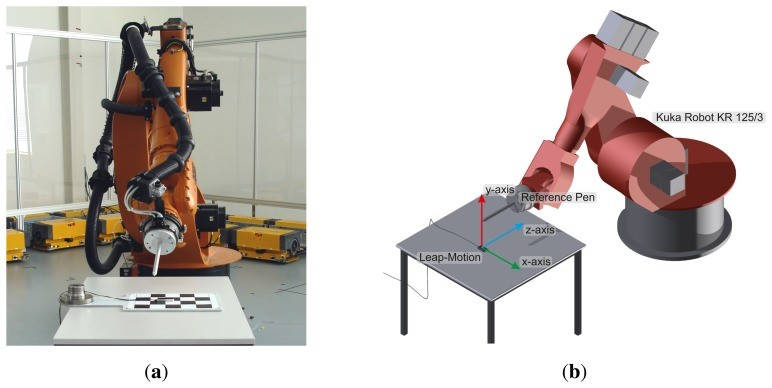
\includegraphics[width=0.8\textwidth]{Anexos/LATEX/chapters/images/Robot_Kuka.jpg}
    %\caption{Evaluación de precisión con robot Kuka 125/3}
    %\small{\textbf{Fuente:} https://goo.gl/yuCTnk}
    %\label{LEAP3}
%\end{figure}

%Usando la precisión del robot como marco de referencia y proceso experimental se muestra que análisis de resultado en precisión y repetibilidad del controlador demuestra un sistema de seguimiento de gestos y posición con precisión submilimetrica, teniendo en cuenta  la posición determinada del  sensor tiene una influencia directa en la calidad del reconocimiento de gestos, el principal foco de atención fue la evaluación de la precisión y la repetibilidad con referencia al hecho de que la precisión de la mano humana en promedio es de alrededor de 0,4 mm, y de forma paralela un robot industrial con un lápiz de referencia permite una precisión de posición de 0,2 mm.